\documentclass[UTF8, 11pt, oneside]{ctexart}

\usepackage{float}

\usepackage{geometry}
\geometry{a4paper,left=2cm,right=2cm,top=2cm,bottom=1cm}

\usepackage{graphicx}

\usepackage{hyperref}
\hypersetup{colorlinks=true, linkcolor=red}

\linespread{1.6}


\def\articletitle{从秦朝到美国,地形图上的龙兴之地都具备一样的特征}

\usepackage{fancyhdr}
\usepackage{ifthen}
\pagestyle{fancy}
\fancyhf{}
\setlength{\headheight}{14pt}
\fancyhead[R]{\ifthenelse{\value{page}>1}{\thepage}{}}
\fancyhead[C]{\ifthenelse{\value{page}>1}{\articletitle}{}}
\renewcommand\headrulewidth{0pt}

\usepackage{tcolorbox}
\tcbuselibrary{skins}


\newcommand{\zd}[1]{\textbf{\textcolor[RGB]{123,12,0}{#1}}} % 重点

\newcommand{\yh}[1]{% 引用
    \begin{tcolorbox}[enhanced,
        frame hidden, interior hidden,
        before skip = 5mm, left skip=10mm,
        borderline west={5pt}{0pt}{gray!50}]
        #1
    \end{tcolorbox}
}

\newcommand{\biaoti}[1]{% 标题
    \section*{#1}
}

\begin{document}

\begin{center}
    \LARGE{\articletitle\footnotemark}
\end{center}
\footnotetext{
    原文出自公众号“远方青木”的文章 《\href{https://mp.weixin.qq.com/s/W8D6dZvRzTkOdMu5JYSe2w}{\articletitle}》
}

中国的地形图上有几处宝地,能称为龙兴之地的那种。

长安城,也就是如今的西安,中国的十六朝古都,位于关中平原的中央位置,秦朝以此为根基席卷天下,刘邦拿下这个地方后四年就灭了楚国,后世隋唐也把首都定在了此地。

\zd{得长安者得天下,为何长安城和其他城池能有那么大的区别?}

打开地形图就知道了,因为长安所在的关中平原是一个非常神奇的地方,这地方四面环山,仅有几处关隘和外界连接,只要少量兵力镇守这些深山里的雄关,就可以保证关中平原的绝对安全,让关中平原可以成为安全生产的大后方。

\begin{figure}[H]
    \centering
    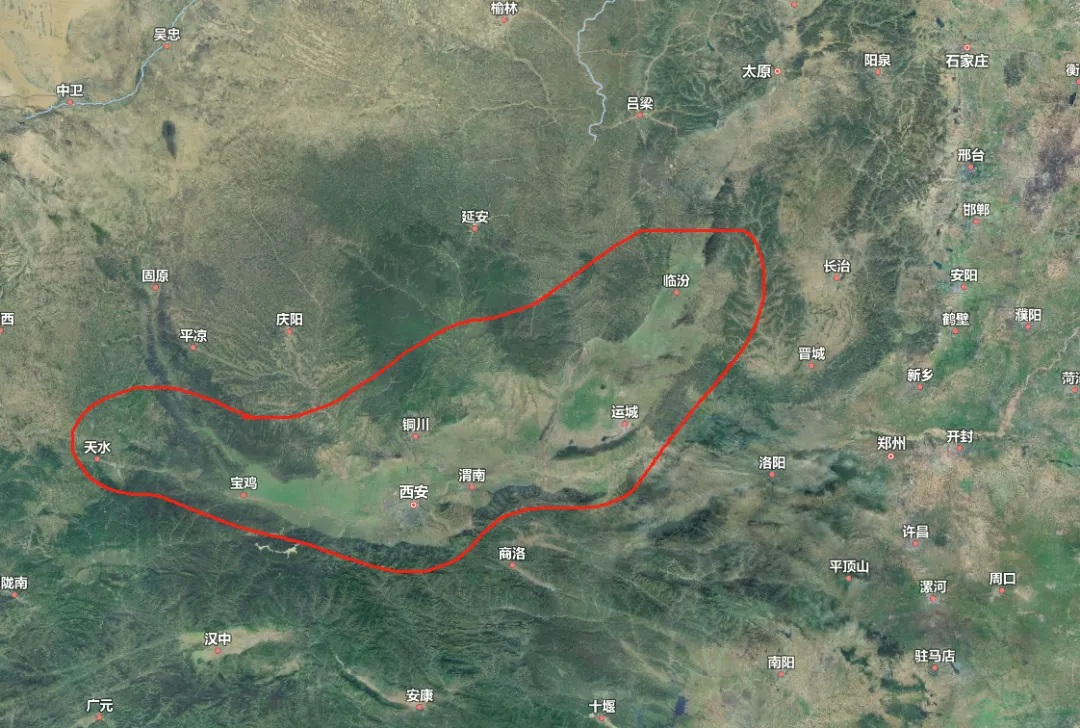
\includegraphics[width=13cm]{2024-08-19-001.jpg}
\end{figure}

函谷关(潼关)、武关、大散关和萧关,共同组成了“四大雄关锁秦川”,战国时期秦国想打其他国家只要出关就能打,今天啃一块地明天啃一块地,但其他六国哪怕合兵在一起都攻不下函谷关。

\begin{figure}[H]
    \centering
    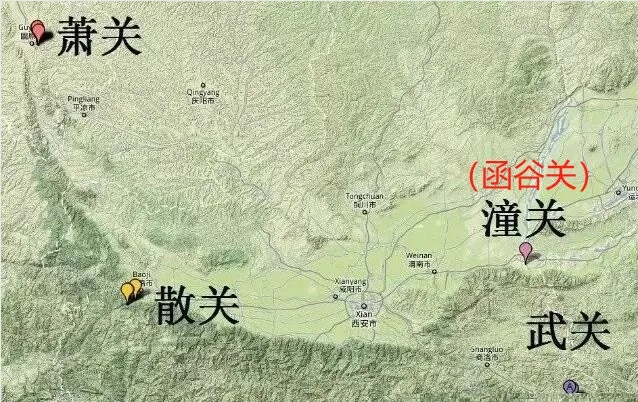
\includegraphics[width=9cm]{2024-08-19-002.jpg}
\end{figure}

因为函谷关的存在,秦国对其他六国立于不败之地,无论输多少次都伤不到根基,可以反复的卷土重来,但其他六国输一次就弱一次,最终被秦国慢慢蚕食。

但哪怕如此,也就等于一个天然的大城墙罢了,是占点地利的便宜,谈不上龙兴之地吧,这些雄关确实易守难攻,但别人不攻,直接从外面封死,你也出不来啊。

这种四面都是高山的平原虽然不多,但也是有不少的,凭什么关中平原可以和其他平原不一样?

\zd{因为黄河流经了关中平原,而且关中平原在黄河的上游,而下游是中原,古代中国的人口和经济的精华所在之地。}

\zd{更神奇的是,中间还卡了个三门峡,运货船想从关中平原出去简单,进来那可就难了。}

\begin{figure}[H]
    \centering
    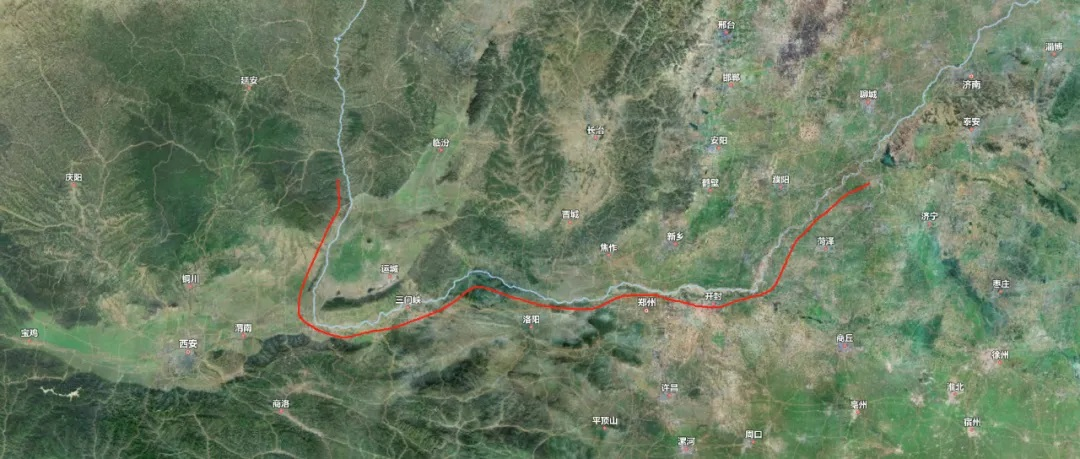
\includegraphics[width=13cm]{2024-08-19-003.jpg}
\end{figure}

打仗就是打后勤,别管多少万大军,一旦断粮饿肚子,饿上几天后全军士兵就不战自溃,而运粮在古代那稀烂的交通条件下是非常困难的事情。

兵马未动粮草先行,古代一个国家想要打仗必须提前把大量粮草运到前线,不仅运输过程损耗极大,而且一旦开战想把粮草从囤积点运到不断前进的军营里也不是那么容易的事情。

但因为黄河的存在,关中平原可以从容在自己腹地囤积粮草,开战后直接让粮船沿着黄河顺流而下就可以了,运输损耗极小而且运输速度极快。

只要你拿下了关中平原,那顺流直下攻打黄河沿岸的城市时,拿下的任何城市都可以直接得到汉中平原的粮草补给,中间的运输几乎是无损耗的,这就是项羽输了一次就补给困难,而刘邦败了多次都好像后勤源源不绝的秘密。

黄河贯穿了中原地区的所有精华地带,而且黄河的存在等于把这些城市连为了一体,兵力粮草都可以共享,互相之间的支援速度也极快。

所以当黄河周边的所有城市都被一个国家占据时,面对可以迅速互相支援,还能集中兵力从任何一点出击的黄河沿线,其他中原城市只有投降一条路,没有丝毫反抗的可能性。

而中原足足有下面这么大,你可以从地形图中看到整个中国大部分地区都是不适合种粮的丘陵和山脉地形,中原是那么凸出醒目的一个巨大冲积平原,所以汉唐时期中国9成的人口和粮食都在中原。

\begin{figure}[H]
    \centering
    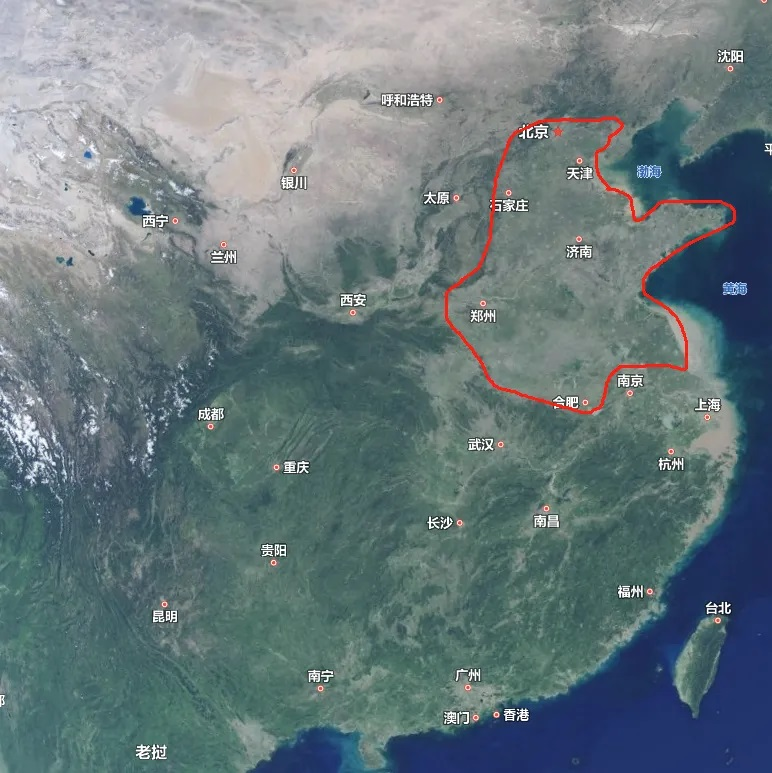
\includegraphics[width=13cm]{2024-08-19-004.jpg}
\end{figure}

\zd{得中原者得天下,而当中原四分五裂没有统一的时候,谁率先拿下了关中平原,谁最有可能统一中原。}

所以关中平原是龙兴之地,所以汉唐都把首都定在长安城,因为中央禁军随时可以从长安出发,沿着黄河行军,迅速镇压中原的一切动乱,古代封建社会的生产力水平下没有比长安更适合做首都的了。

\zd{在中国还有一个地方也堪称龙兴之地,其地形和关中平原高度相似,那就是成都平原,也就是蜀国占据的益州。}

诸葛亮在草庐里建议刘备先取荆州和益州,然后夺取天下。

此时的关中平原和中原已经基本被曹操统一了,拥有了无穷的人力和粮草,其余势力理论上只有投降一条路了,但诸葛亮认为如果刘备能拿下荆州和益州,那还有翻盘曹操的希望。

成都平原是诸葛亮计划的核心,这里和关中平原类似,四周都是高山,拿下之后易守难攻,可以从容不迫的在益州囤积兵力和粮草,外界很难攻入。

而成都平原是长江的上游,占了这里之后可以随时集中益州的兵马粮草,源源不断的攻击下游。

下游第一站就是荆州,这里也是一个平原,叫江汉平原,占了这里之后下游的东吴不足为虑,因为上游打下游就是很简单,而荆州又在益州的下游,受制于益州。

所以刘备镇守益州,关羽镇守荆州。

拿下益州后,刘备还可以向北打汉中平原,拿下汉中平原后以这里为前进基地,伺机攻击关中平原。

一旦关中平原被刘备拿下,则中原不保,曹操将会失败,而从历史来看,诸葛亮从汉中平原出发攻击关中平原虽然屡屡失败,但并非没有成功的可能性。

而在占领益州的同时占据荆州,是因为从荆州向北出兵虽然无法占到顺流而下的运输便利,但可以直接攻击中原,这样可以牵制调动曹操军队,因为只有曹操军队被大量调离关中平原的时候,益州的部队才有攻下雄关进军关中平原的可能性。

如果整个中原的兵力都被曹操调过来堵在益州门口,那诸葛亮是打死都出不来的,所以必须有部队在荆州攻击中原。

\begin{figure}[H]
    \centering
    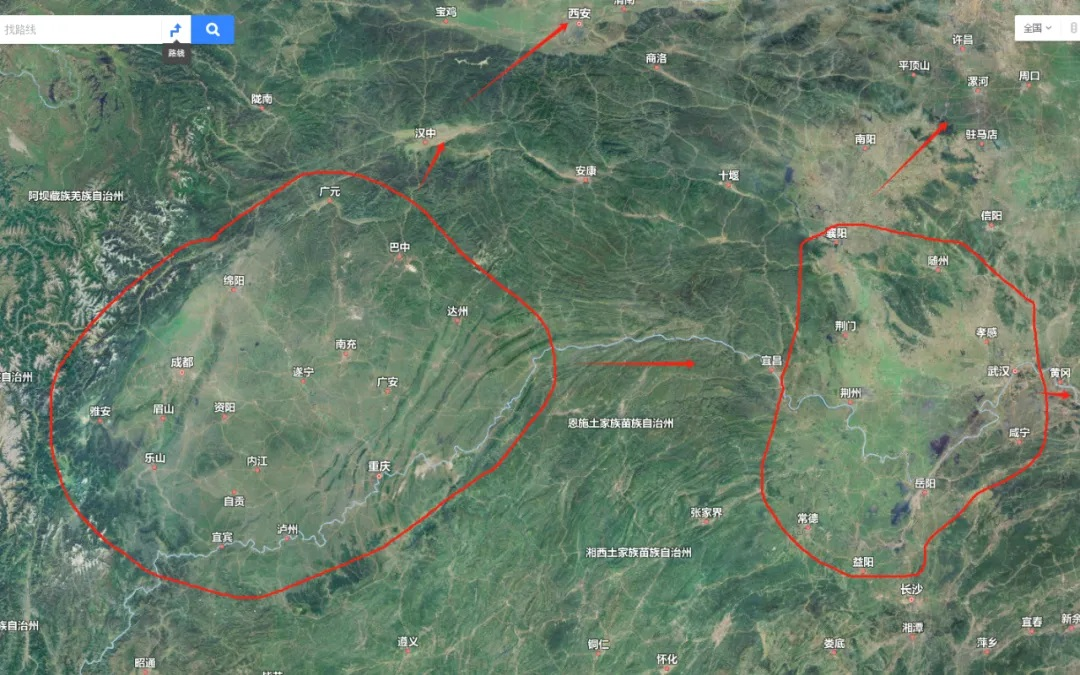
\includegraphics[width=13cm]{2024-08-19-005.jpg}
\end{figure}

这个规划非常完美,而且确实一度接近成功,关羽水淹七军威震华夏,汉中平原被刘备直接拿下,曹操的确可能被翻盘。

但因为东吴的偷袭,关羽兵败身死,荆州被东吴夺取,蜀国的战略直接少了一条腿,导致最后曹魏统一了天下,蜀国灭亡后东吴也跟着灭亡。

这并不能完全算是东吴短视,因为按照诸葛亮的计划走,同时占据荆州和益州的蜀国确实可能击败曹魏,但只要腾出手来随时可以消灭东吴,与其如此那吴国还不如拿下荆州增强自己。

而诸葛亮反对利用上游优势沿着长江攻击吴国,长期从从汉中平原死磕关中平原,主要理由就是沿着长江灭了吴国没有用,还不如保留力量让吴国牵制魏国。

\zd{先得关中平原者得天下,而先得成都平原者未必,最大原因就是黄河的下游是中原,而长江的下游只有荆州所在的江汉平原,双方的体量差距巨大。}

如果诸葛亮能幸运的打下关中平原,则有翻盘希望,但哪怕诸葛亮幸运的打下整个吴国,也没有翻盘希望,这两者的差别太大了。

假设蜀国以极小的代价拿下了吴国,然后控制长江的蜀国和控制黄河的魏国单挑,那么除核心的龙兴之地关中平原和成都平原的争夺外,双方的战场将围绕襄阳一带,以及整个江浙平原进行。

\begin{figure}[H]
    \centering
    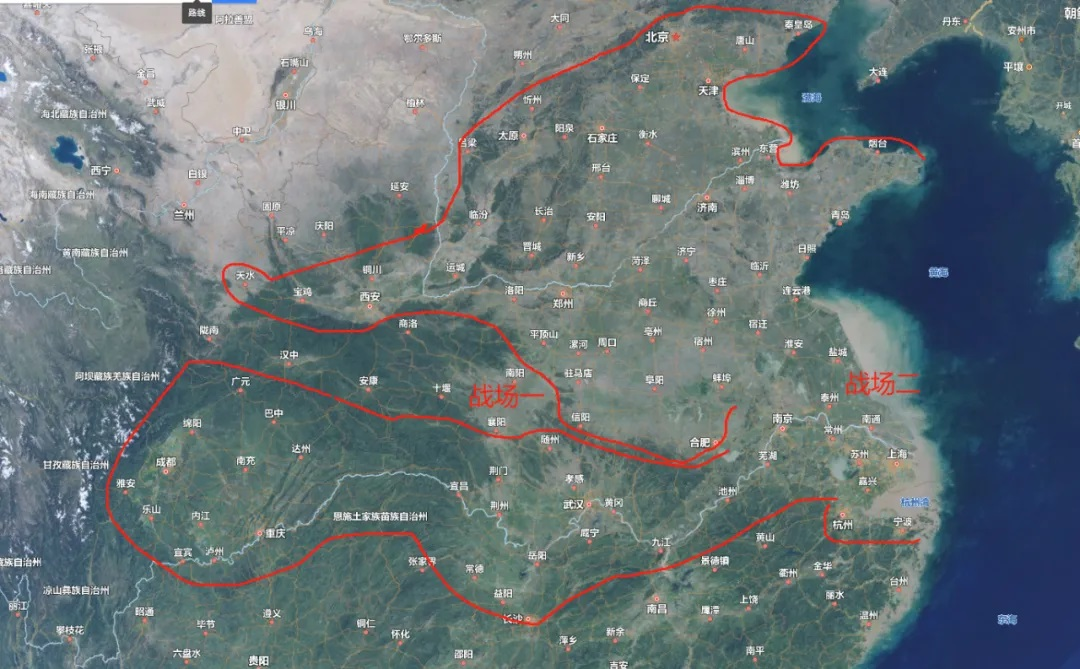
\includegraphics[width=13cm]{2024-08-19-006.jpg}
\end{figure}

但很明显,双方的体量差距太大,平原厮杀到最后就是拼人力物力,基本谁地盘大谁赢。

黄河下游的中原太大,而长江下游平原太少,大部分地区都是“两岸猿声啼不住”的景色,所以拿下关中平原的收益远远大于拿下吴国,而且拿下吴国是肯定有兵力损耗的。

\zd{因此关中平原是最强的龙兴之地,成都平原是次强的龙兴之地。}

如果地球自然环境没有发生变化的话,那整个中国封建时期的首都都会是长安城。

但在唐朝中后期,小冰河时期降临,整个地球的气温大幅下降,北方降雨量大幅减少,曾经富饶的西域直接被埋入了沙漠,而关中平原虽然没有变成沙漠,但降雨量也大幅下降。

秦汉时期是八水绕长安,长安城附近河流密布气候宜人,但到了唐朝中后期长安城附近的河流全部断流,不仅八水绕长安没了,甚至连长安城的护城河都干涸了。

少了护城河还不算什么,可怕的是不仅河流大面积消失,整个关中平原的粮食产量也大幅下降,已经缺粮缺到难以支撑长安城人口的地步了。

唐朝有两个首都,一个是长安一个是洛阳,之所以在定都长安城的情况下还要建都洛阳,就是因为要“迁都就食”。

\zd{大唐王朝供不起长安人吃饭了,因为缺粮,而把粮食从黄河下游运到上游太困难了,三门峡那一段太险峻了,下来简单上去太难。}

唐朝时期整个关中平原频频爆发饥荒,一旦遇到粮食不足,那把长安人迁移到洛阳吃饭的成本,是显著低于把中原的粮食运到长安的。

唐朝君臣到洛阳就食是一种常态,整个唐朝发生过十余次大规模到洛阳就食的事件,每次不仅皇帝和文武百官会离开长安到洛阳,所有的宫廷女眷和禁卫军都会到洛阳,随行的还有大量长安民众。

等关中平原的粮荒退去,攒够了一部分粮食,那整个朝廷再返回长安,因为长安城更安全,洛阳毕竟在函谷关保护之外。

\zd{为方便唐朝君臣反复到洛阳就食,唐朝沿着长安-洛阳的古道修建了16所行宫、21所驿馆,为唐王朝的频繁大规模就食迁移提供后勤保障。}

为什么地形如此完美的长安城,在唐朝之后的王朝里被放弃成为首都,你看看这不堪回首的就食历史就知道了,堂堂首都连饭都吃不上了,这怎么当首都。

而且关中平原之所以能当龙兴之地,就是因为这里天然自产粮食,可以源源不断给下游输送军粮。

但如果关中的粮食都无法自给,那将来开战怎么给下游输送军粮?甚至别人只要把函谷关一封,不让外界运粮进去,那关中就直接因为缺粮而爆发内乱了。

后来因为更加干旱少雨,黄河甚至频繁断流,船只无法通行,关中平原那不可撼动的战略意义就更小了。

\zd{唐朝灭亡后是五代十国,之所以乱成这样就是因为没有一股势力可以轻松定鼎天下,而长安城在五代十国期间被多股势力夺取过,每一股夺取长安城的势力,都做不到像秦汉唐时期那样可以凭借关中平原轻松席卷天下,得长安者得天下的神话再也无法复现。}

地势没变,但关中平原不再是大粮仓了,所以优势锐减,长安城如同鸡肋在五代十国的实战中被反复证明,这一切都是因为唐朝时期的气候剧变。

十六朝古都长安城,最终被封建王朝放弃。

唐朝之后的宋朝,选择了在开封定都。

其思路还是利用黄河轻松连接沿线城市的人力物力,形成相对于中原其他地区的碾压优势来定都,而且开封地势平缓,本身就在中原的平原地区,从下游运粮非常容易。

\begin{figure}[H]
    \centering
    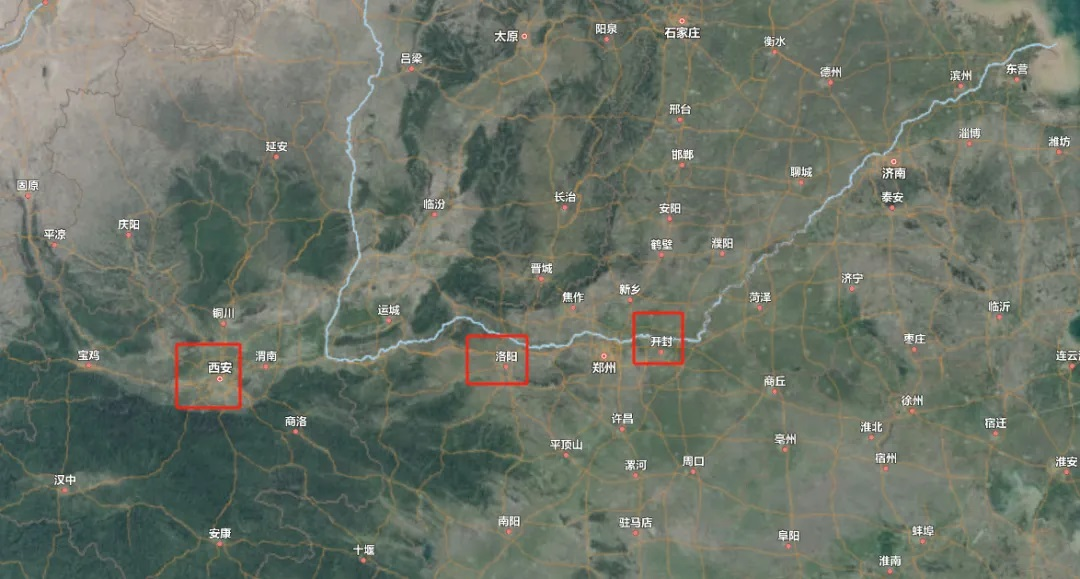
\includegraphics[width=13cm]{2024-08-19-007.jpg}
\end{figure}

这种思路实际上是把中原当成了一个巨大的关中平原,因为中原地区三面是山一面是海,统一中原巨大的人力物力后,反推上游并不困难。

争夺天下的核心是夺中原,而天下既然已经统一,那最核心的诉求当然是保中原,那定都在中原的核心位置自然是正确的选择。

\zd{这思路没错,但封建王朝对军队的控制力太弱了,离开皇帝百里后军队的战斗力就急速下滑,离开皇帝500里的军队基本都在摸鱼划水,皇帝这个老板只要看不见那军队就不干活。}

所以北京所在的燕云十六州,虽然有宋军把守着雄关,但游牧民族还是轻松打破,随后凭借中原的一部分建立了金朝。

失去燕云十六州的天险后,金宋两国在中原疯狂厮杀,但金朝有马宋朝没有,在中原厮杀宋朝吃了大亏,最终宋朝战败,开封陷落北宋灭亡,南宋被赶到了长江附近凭借群山据守。

元朝灭亡金朝后又灭了宋朝,随后被明朝消灭。

吸取宋朝教训,明朝最终定都北京,天子守国门。

\zd{皇帝离开了老板室,亲自在大厅工位里坐着,随时监督中央禁军支援大同-张家口-承德-秦皇岛这四大关隘,确保中原无忧。}

\begin{figure}[H]
    \centering
    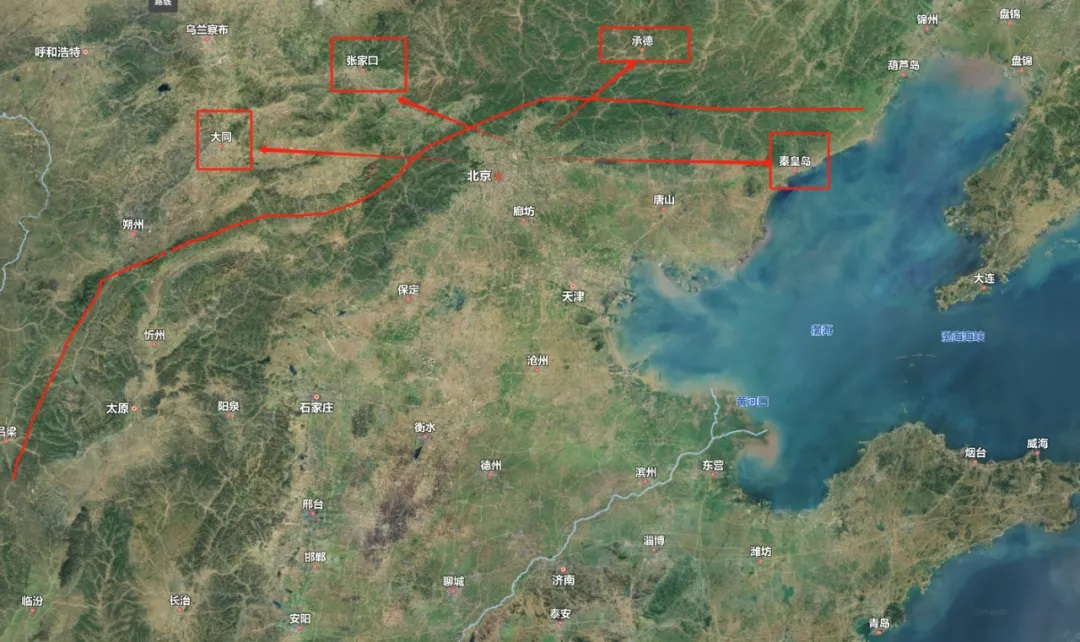
\includegraphics[width=13cm]{2024-08-19-008.jpg}
\end{figure}

这四大关口之外都是险峻的群山,军队根本无法通行,所以皇帝带着禁军把守北京后,游牧民族攻关时面对的将是汉族的最强武力。

这样做中原的北面确实无忧了,但南边就不要了?

刚才的地形图大家都看了,中原的南边全是山,越向南的山越险峻,明朝向南一直打到了海边,西南方向到了云南附近面对重重叠叠的巨大山脉人都麻了,勉强向前推到越南附近后就撤了。

这里离开皇帝太远,军队战力下滑的太厉害,攻是攻不动了,但建点雄关,外面也根本攻不进来。

向南没问题后,再看看其他方向。

中原向西,全是山,没有具备威胁度的敌人。

中原向东,全是海,没有具备威胁度的敌人。

唯一能威胁中原的就是草原,因为草原没法种地,农耕王朝统治不了,打下来也要不了,所以就定都北京,防备游牧民族就够了。

\zd{这时候整个中国就形成了一体,四面八方都很安全,可以随时聚集内部的人力物力向外攻击任何一个点,而外界想打中国则困难的多。}

\zd{以中原为核心,以一圈群山和大海为屏障,中国形成了一个巨大的龙兴之地,对周围任何国家都具备巨大的战略优势,因此明朝把自己的领土推到了农耕民族能控制的极限。}

能种地的地方,都是明朝的,直到距离首都太远实在控制不了为止。

限制中国领土的是封建时代那落后的通讯能力和统治能力,以及陆地运粮实在太困难了,离开长江黄河以及其他内河运粮通道后攻城略地成本太高,否则依托这个巨无霸版本的“关中平原”,中国能席卷整个亚洲。

\zd{也因此中国文化中一直有大一统执念,无论哪股势力兴起都要大一统,因为中国这种地形大一统后就能用驻扎在关键关隘上的极少军队形成巨大的军事威慑,确保所有人的安全,少一块都无法达成这种神奇的效果。}

\zd{经济基础决定上层建筑,因此这种地形下诞生的政权,其文化一定是大一统的,因为大一统相当于所有人都可以出最少的钱买到最安全的国防。}

清朝的龙兴之地是东北,这不是因为清朝兴起于东北才称之为龙兴之地的,而是因为东北确实具备龙兴之地的条件。

当然这个龙兴之地只适合清朝,因为清朝很特殊。

在中国历朝历代的文化里,东北都没什么特殊的,因为这地方不仅位于偏僻边角而且无险可守,只能等着被统一中原的政权统一,断无反推的可能,当不了龙兴之地。

清朝创始人努尔哈赤是农耕系统出身但不执行彻底的农耕,虽然依靠给明朝称臣起家,虽然一直为明将李成梁冲锋陷阵,但因为东北特殊的地形,努尔哈赤没有贯彻农耕思维的本钱,像明朝那样单纯种地必死无疑,因为东北大面积的和草原接壤,无险可守。

所以虽然农耕思维深入清朝政权骨髓,但因为东北的大环境,起家的时候被迫大面积的和游牧思维融合。

草原即便被农耕政权击败也是无法被农耕政权统治的,但清朝起家的环境恶劣,想活就必须统治草原,因此发展出了一套满蒙共治天下的理念。

这个共治天下可不止是说说,满清皇宫里都是蒙古后妃,然后满清的格格大量嫁给蒙古王公,利益分配上蒙古只负责军事,不交税,每年净拿军费。

搞定草原政权后,东北就突然成了“龙兴之地”。

虽然没有群山保护,但当草原上全是自己人后,东北这地方就没了外敌。

山脉的阻断是双向的,明军同样无法凭空越过山脉攻击另一侧,所以明军的行军路线是可以预测的,只能从山海关出东北,然后也只能沿着固定路线前进,其他地方不行,这就是山脉限制的好处。

南边是朝鲜,和东北有群山阻隔,夺了关口后这个群山就反过来成了阻碍朝鲜出兵的天险。

\begin{figure}[H]
    \centering
    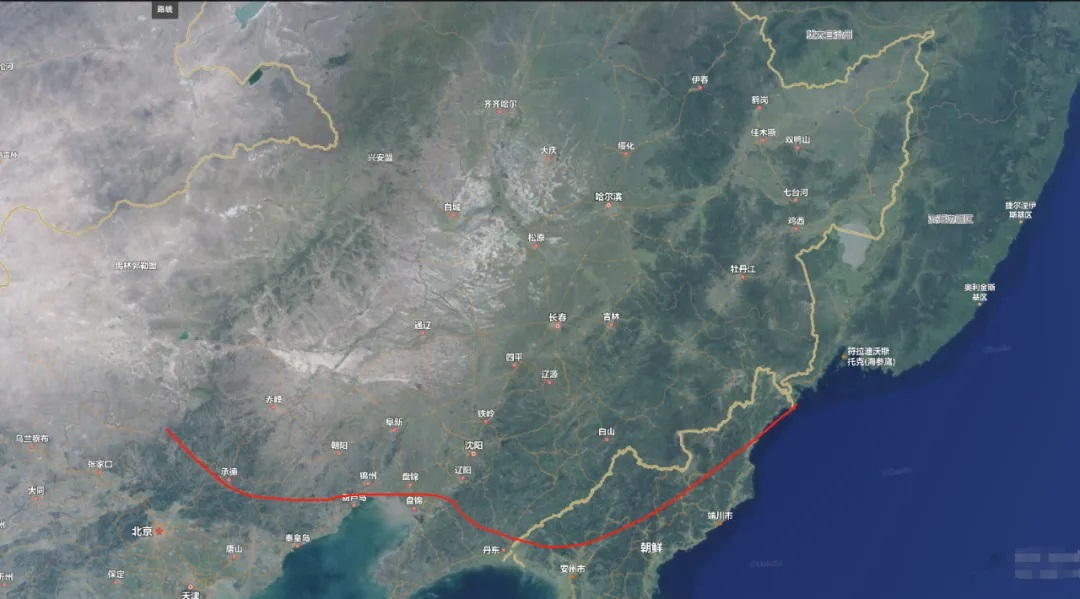
\includegraphics[width=13cm]{2024-08-19-009.jpg}
\end{figure}

东边是海,空无一人。

北边是无人区,彻底的无人区,虽然今天看起来和俄罗斯接壤,但当年清朝是一直向北推进到了人类能生存的极限,能能看到的所有活人都抓过来当八旗兵了。

当时东北的北方别说政权,连活人都没有,当然就没有外敌。

因此东北就成了一个稳固的大后方,可以安心搞生产,反复攻击明朝,成了类似关中平原和成都平原一样的“龙兴之地”。

但即便如此东北一地的力量还是太弱了,末年的明朝都腐化成那个样子了,背靠中原和群山里的雄关,清朝依然一点办法都没有,最终还是明朝内乱自己灭亡了清军才得以入关的。

从这个角度说,即便扫清了后方隐患并统一了草原,东北依然不够格称之为“龙兴之地”。

但明朝因为我上面说的原因,把首都定在了北京,东北边上。

因为明朝的首都在北京,所以东北弥补了实力不足的最后一环,最终成为了完美适合清朝的“龙兴之地”。

\zd{明朝可以防御清朝无数次,但只要被清朝抓住一次机会打下了北京,那中原就直接崩溃,席卷中原后,清朝就无可阻挡的会统一天下。}

\zd{从这个角度说,东北确实是龙兴之地,但只适合清朝这种农耕游牧两头吃的特殊政体,同时要求中原的首都必须定在北京。}

而清朝这种政体堪称是农业时代人类政权的极致,全球都没有诞生过如此离谱的政权,如果不是欧洲爆发了工业革命直接跨了一个技术时代,农业时代的任何人类国家都打不过清朝,因为农业时代除清朝之外的所有人类国家要么是农耕要么是游牧,没有能兼容的政权。

明朝在自己的控制力极限范围内,把所有能种地的地方都变成了中国领土。

而清朝不仅控制力极限范围远远大于明朝,占了所有能耕地的地方,而且在明朝的基础上,把所有能放羊的地方都变成了中国领土。

清朝在东西南北四个方向上都打到了无人区,放羊都很难生存的那种,奠定了今天中国领土的基础。

清朝的核心还是中原,但外围保护远远不止群山和长城了。

在东边,大海是中国的边界。

在西边,新疆和中亚地区之间的戈壁沙漠等无人区是中国的边界。

在北边,农业时代完全不适宜人类居住的冻土层无人区是中国的边界。

在南边,喜马拉雅山和云南那超级险峻的群山和无人区是中国的边界。

任何能威胁到清朝的外敌都不存在了,因为靠着安全的中原腹地搞生产,清朝可以不断的大吃小,滚雪球一样越滚越大,直到自己制度统治力的极限。

\zd{清朝只会亡于内乱,绝不会亡于外敌,这是清朝士大夫的统一认知,因此清朝对内部的汉民严防死守。}

他们这么认为也没错,因为清朝的版图太完美了,农耕文明政权的极致,任何外敌入侵中国不仅会顿兵于雄关天险之下或困于无人区之中,而且会立刻遭到整个中国的合力反击,同时中国那稳固的大后方会源源不断的生产兵力和粮食,外敌很难破坏,在雄关天险或无人区那里和整个中国拼后勤显然是一个注定失败的选择。

因此清朝士大夫们认为中国对外是无敌的,只有内乱这一个隐患。

\zd{直到欧洲发生了工业革命,然后“有敌自海上来”。}

中国自古以来就没有外敌通过海洋前来,而且自己出海也极度困难,通过海洋大规模运送兵力是不可能的事情,当年元朝如日中天的时候试过打了一次日本,直接被台风给团灭了。

所以古代中国从不考虑政权被海洋来敌灭亡的可能性,因此老祖宗在大一统的时候,打到海洋就算完美了,因为后方安全了,默认海洋方面不可能大规模来敌。

直到欧洲步入工业时代建造了钢铁巨舰,让大海变成了通途。

\zd{从此中国这个完美的“龙兴宝地”出现了一个巨大的缺口,所有临海的位置都可能来敌,而且敌军依靠军舰行军速度极快,这情况比古代所有关隘被攻破还要糟糕。}

1840年鸦片战争的时候清军被英军耍猴一样玩,漫长的海岸线英军想打哪里就打哪里,上个月还打广州呢这个月就到上海了,而清军想把部队从广州调集到上海,光行军都要花半年。

这情况和当年关中平原的军队粮草可以顺黄河而下的情况高度类似,但情况反过来了,这次是中国被凭借海洋优势的外敌轻松吊打。

别说技术和制度都有代差,就算技术和制度没代差,光行军和后勤这么巨大的劣势,那清朝都必输。

海洋从安全屏障变成了外敌通道,直接让中国所有的沿海区域都无法成为安全的后方基地。

然后就是工业时代巨大的生产力发展,让北方的冻土层也可以通行人类军队了,虽然今天俄罗斯的远东区域依然不适合人类居住,每年需要花费大量卢布补贴居民生活,但通行军队还是做得到的。

这让中国的安全边界大大收缩,北面那曾经的无人区不再绝对安全,至少要缩到群山屏障才适合抵挡,而随着飞机大炮技术的跨越式发展,这些群山屏障阻止陆军的能力也大幅下降。

\zd{所以今天的中国地缘环境并不好,到处都需要派兵设防,除了背靠喜马拉雅的大西南山区,感觉没有地方是绝对安全的。}

\zd{不是老祖宗没有考虑国家安全,而是老祖宗已经做到了他们认为的极致安全,曾经的古代中国只要统一,那全国到处都是安全的,外敌从哪都进不来。}

但工业时代的生产力飞升太离谱了,才导致如今中国的版图不完美了,以至于没有安全感。

工业时代的龙兴之地,是美国。

这个地方太完美了,一边是太平洋一边是大西洋,周边虽然还有加拿大和墨西哥等邻国,但这些国家太弱小了,对美国完全构不成陆地威胁,能击败美国的强敌全部都被两大洋那茫茫远的距离所阻挡。

整个北美洲大陆,都可以被视为曾经的“关中平原”,美国可以在这里安心的搞发展,不断积累实力,外敌攻不进来。

\begin{figure}[H]
    \centering
    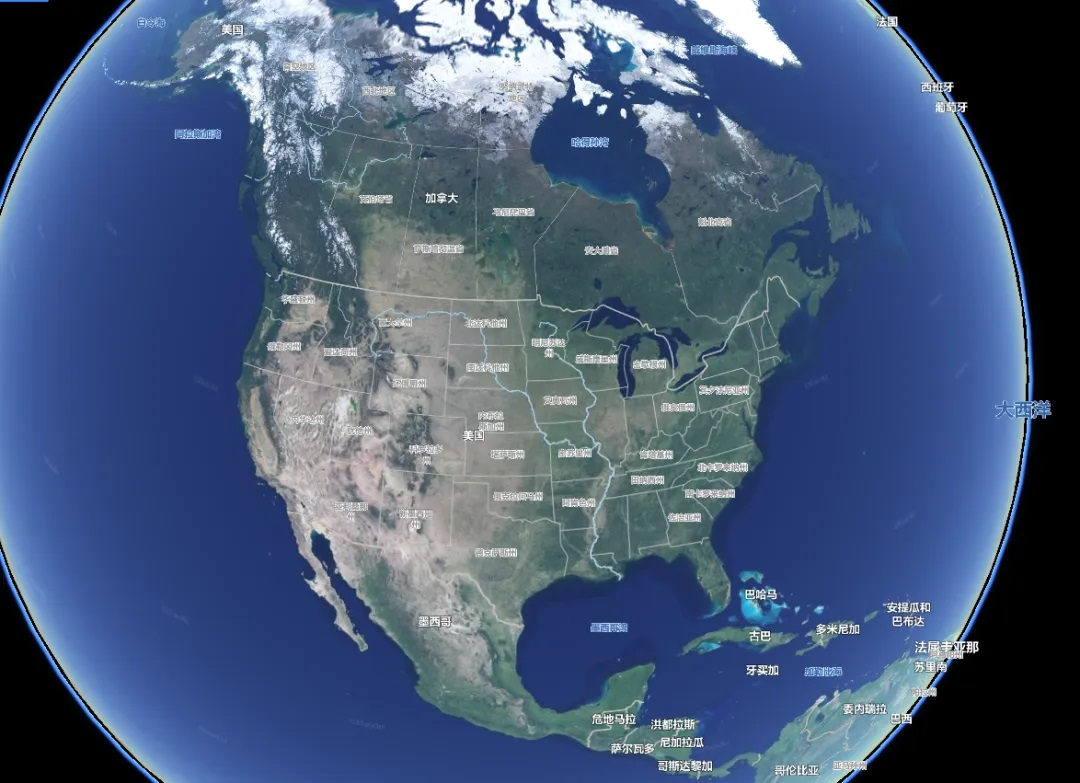
\includegraphics[width=13cm]{2024-08-19-010.jpg}
\end{figure}

海洋没有上下游之说,所有海军都具备平等的通行权,但美国拥有着世界最强海军,其规模曾经相当于其他所有国家之和,所以这两大洋成了单方面保护美国的屏障,对其他国家而言则只是美国单方面运兵的通道。

通过足够强大的海军,美国强行在海洋上制造了上下游的区别。

\zd{这是绝对的龙兴之地,可以说是龙兴宝地,依托这块宝地,美国理论上可以轻松的席卷世界,不断大吃小,对地球实现大一统。}

整个地球对于美国,就和当年四分五裂的中原对于关中平原是一样的,集合关中平原的人力物力,沿着黄河顺流而下就可以轻松席卷中原。

事实上美国也确实做到了,苟到两次世界大战后的美国确实具备了席卷世界的能力。

但美国的制度统治力太弱,无法消纳和统治其他地区,别说席卷世界,送上门求融合的地区一大堆,美国都不要,因为要了自己内部就不稳固了。

送上门求融合的中型国家菲律宾,美国不要,因为人口1亿,送上门求融合的波多黎各,到今天人口才300万,美国还是不要。

\zd{美国接纳为领土的几个岛国,人口都在十几万左右,而且在合并领土前其人均居民收入就超过了美国,这两个条件同时满足是美国愿意进行领土融合的最低要求。}

\zd{从建国第一天开始,美国就只要地不要人,领土能变这么大是因为印第安人被杀光了,必须同时接纳上面土著的地,美国一块都不想要。}

从地缘战略上来说,美国已经达到了可以统一全球的标准,美国当年只要愿意融合,不断大融小,甚至小半个地球都能传檄而定,但美国的领土范围被自身的制度统治力给限制了。

制度决定了美国的领土只能这么大,而且这已经很幸运了,美国当年恰好可以屠光印第安人才能有这么大的领土,和美国同文同种的英国当年占了半个地球,但实际统治的领土从头到尾就只有自己那个岛,因为自身统治力太弱,制度决定了其领土范围无法扩大。

所以如今的美国就是巅峰了,虽然给了龙兴宝地,但美国已经扩不动了。

\zd{任何国家都不可能永远保持巅峰,所以美国地缘优势再好,也就这样了。}

\zd{因此我们需要再看看地球上还有没有第二块龙兴宝地。}

农业时代的中国是龙兴宝地,而在工业时代成了四战之地,处处漏风。

但,事在人为,先天条件不好,可以人为修补。

喜马拉雅山和中亚无人区的阻隔依然有效,所以这两个方向我们依然是安全的,只有北面和海洋两个方向的防御需要修补。

自苏联解体后,中国就没有拿俄罗斯当过对手,反而一直在笼络俄罗斯,因为美国一定会打击世界第二,但俄罗斯没有这个需求。

而中国北方的冻土区虽然在如今的工业时代可以勉强住人,但生存还是很难,所以中国和俄罗斯没有太大的利益冲突,因为中国的北边和俄罗斯的远东都没什么人住。

俄罗斯的经济命脉在莫斯科那边,位于东欧区域,和中国十万八千里。

而中国的经济命脉在东南沿海,位于东亚地区,和俄罗斯十万八千里。

双方的经济命脉没有冲突,甚至互补,所以如果可以和俄罗斯“共治天下”,那俄罗斯可以成为中国在北方的巨大屏障。

从90年代开始,俄罗斯就一直想和欧洲修好,但这怎么可能呢,美国肯定反对,中国也不会支持,而俄罗斯的经济命脉地区和欧洲的经济命脉地区靠的太近了,双方才是真正的邻国。

中国和欧洲这种远到绝对不可能有领土冲突的国家,才可能真正修好,所以哪怕美国一直煽动欧洲反华,我们也是坚定和欧洲保持良好关系。

但美国还在同时煽动欧洲反俄,而欧洲和中国关系越好,美国煽动欧洲反俄就越容易,俄罗斯就越难和欧洲处关系。

另一端,俄罗斯越难和欧洲处关系,就越依赖中国。

所以俄乌战争中国不插手,虽然我们支持俄罗斯,但俄乌战争我们就是不插手。

只要持续和欧洲修好,只要持续保持中立,俄罗斯就会持续的向中国靠拢,利用种种利益绑定,参考一下当年清朝政策,让俄罗斯认定跟着中国混能“共治天下”,跟着其他人都没啥好下场,单独自己也无法出头,那不仅北方威胁全消,甚至还凭空多了一个巨大屏障以及同盟军。

\zd{从90年代开始,中国就认定俄罗斯早晚会倒向中国了,这和俄罗斯的意愿无关,和地缘利益的必然性有关,俄罗斯试图撇开中国和欧洲修好,只是挣扎一下这个结局而已。}

因为这30年,中国在拼命发展海军,陆军反而不断裁剪规模,这说明我们早在30年前就认定俄罗斯不是敌人了。

\zd{我们的安全屏障只剩一个方向还有缺口,那就是海洋。}

\zd{东南沿海城市很不安全,不仅不是能支撑中国前线的大后方,甚至如果将来遇到战争自己就是前线,偏偏这里是中国的精华所在,经济命脉地区。}

而工业生产比农业生产还怕战乱,本国经济命脉前面没有安全屏障,任何政权都不会有安全感的。

\zd{我们要把这个安全漏洞封上,就要找到海洋里的“函谷关”。}

虽然海洋是通途,但军舰是需要补给的,燃油弹药和淡水饮食都需要随时补充,短距离内军舰可以到处乱窜,但长距离内军舰的行军路线是固定的,必须沿着补给线前进。

唯一可以威胁中国的只有美国,所以只要解决掉美国海军的威胁,其他国家的海军不足为虑。

美国灭不掉中国,即便大家都没有核武器美国也灭不掉中国。

但中国也灭不掉美国,即便大家都没有核武器中国也灭不掉美国。

因为双方的国土距离太远了,隔着一个太平洋,长达1.2万公里,人类目前的技术无法无视太平洋那遥远的距离。

所以太平洋就是海洋上的天险,和陆地上的无人区可以阻隔军队是一个道理。

打开地形图,就可以轻易发现这个天险上的关隘,那就是韩国、日本、台湾、菲律宾以及南海。

\begin{figure}[H]
    \centering
    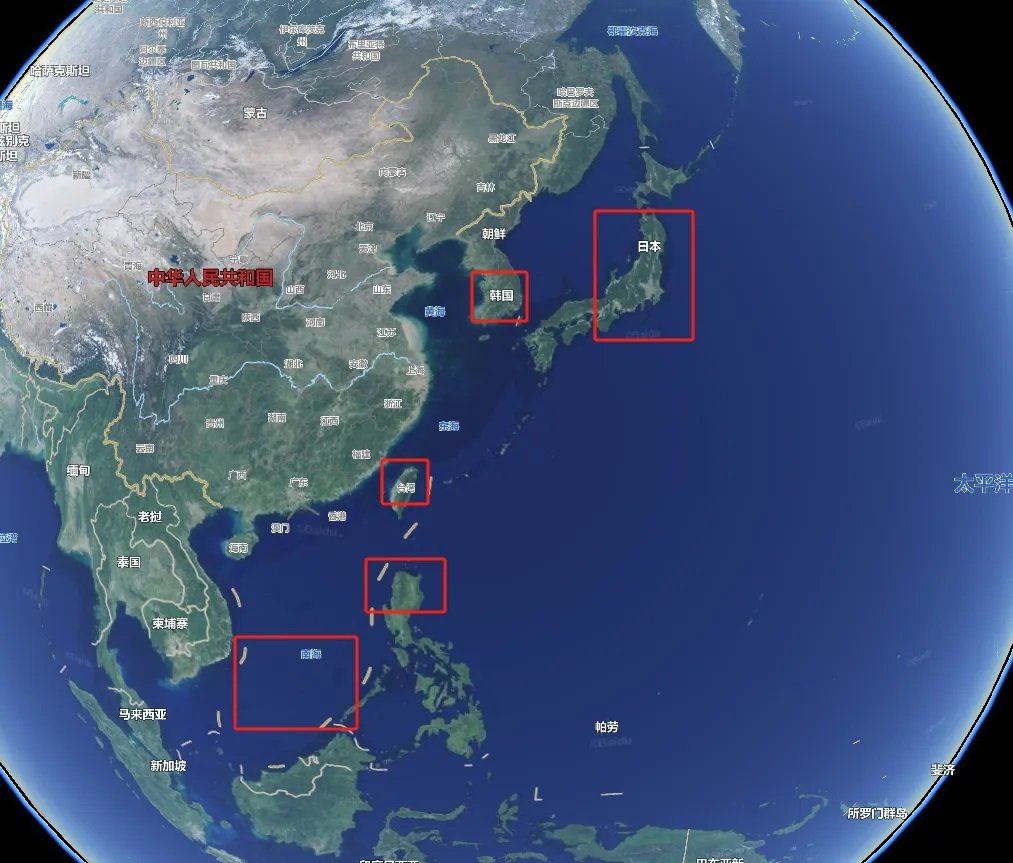
\includegraphics[width=13cm]{2024-08-19-011.jpg}
\end{figure}

这里是一个个的囤兵点,也是海洋关隘,中国新时代的“函谷关”。

如果这里有美国驻军,让美军在这里驻扎并囤积弹药粮草,那中国的东南沿海就不可能是稳固的大后方,因为美军从这里出发可以随时攻击中国的东南沿海。

但如果这里没有美国驻军,让美国想攻击中国的东南沿海就必须从美国本土出发,那想打中国的东南沿海就困难的太多太多。

如果这里不仅没有美国驻军反而有中国驻军,那美国海军想攻击中国,不仅需要从美国本土出发途径万里之遥,而且会被守在这里的中国驻军以逸待劳。

只要守在日韩的中国军队还在,中国的东南沿海是安全的。美国唯一能攻击中国本土的方式就只剩下了洲际导弹,而这种东西是不可能打败一个国家的,哪怕装了核武器都是,想真正击灭一个国家是必须登陆作战,逐个城市占领,彻底扫清抵抗力量的。

而且哪怕用了装载核武器的洲际导弹,中美双方也是平等的。

而菲律宾和南海也是一样的道理,掌握这里可以给东南沿海城市留出足够的安全空间。

菲律宾距离中国东南沿海最近处650公里,南海边缘距离中国东南沿海最近处2000公里。

虽然人类的技术远远比古代发达,但遥远的距离还是一样可以带来安全,

如果这里都被中国海军控制,那外敌想袭击中国,就必须攻克日韩台菲至少一个点,否则距离中国东南沿海太远,普通火力够不着。

这四个点,就是海洋里的四大关隘。

但中国近代国力太弱了,海军实力约等于零,所以这对中国极其重要的四大海洋关隘全部都是美国的势力范围。

\zd{这就相当于虽然关中平原是我们的,但四大雄关全都是美国的,那整个关中平原就谈不上安全,也不可能称之为龙兴之地。}

函谷关、武关、大散关和萧关全都被美军占领,随时可以攻打关中平原,你想抵抗也只能在关中平原上抵抗,输赢先不说,关中平原肯定是被打烂了。

“四大雄关锁秦川”,中国如今是被锁的那个。

\zd{所以我们拼命建海军,在台湾和南海问题我们寸步不让,因为这甚至不是简单的领土问题,实际上这事关中国这块地到底是不是一个完整“关中平原”的问题。}

\zd{解决不了自身安全问题,四大雄关掌握在别人手里,那中国就不可能登顶世界之巅,以后的世界就算诞生了机会也不是中国能拿的。}

而更麻烦的是,这四大雄关只要美军还掌握一个,中国的东南沿海就依然谈不上安全,美国依然可以顺着自己掌握的那个雄关进攻关中平原。

所以我们不断积累实力,在南海和台湾问题上引而不发,就是在找机会,一个能同时把美军势力清扫出日韩台菲的机会。

能达到这个效果,为中国树立海洋屏障,付出代价才是值得的,否则就不值得,单纯一个台湾不值得中国付出代价,因为拿回来不仅要冒着战争风险,而且即便成功也无法解决中国东南沿海城市的安全问题。

甚至少清扫一个美军据点都不值得中国付出代价,如果我们决定付出代价开战,那一定要同时拿下四大雄关,彻底保证中国沿海安全。

从法理上看是有可行性的,因为日本是二战的战败国,和中国是有协议的,中国军队可以合理合法的驻军日本,只要赶走美军就行。

中国驻军韩国不合适,但韩国和朝鲜从没签过停战协议。

南海一直是我们的,从古至今都是我们的。

菲律宾有点麻烦,法理无据,所以需要菲律宾自己折腾出充足的理由,因此菲律宾军舰坐滩仁爱礁已经24年我们都没管,而且这还不够,需要等未来大变时菲律宾自己做出大的错事。

最坏考虑,菲律宾永远骑墙,未来跟着美国也是只出工不出力,绝不彻底站队,绝不给中国理由,那在其他地方和美国冲突的时候也是可以一并把美军驻菲律宾的军事基地给赶走的,其他的再慢慢谈。

\zd{这些是未来中国必须做的事情,因为给本国经济命脉建造足够的安全屏障是中国的本能,我们可是一个为了能安全搞生产愿意修长城的国家。}

把美军驱离出这四大关隘,对中国的好处极大,但对美国的坏处也是极大。

因为这四大关隘是美国在东亚的战略支点,美国就是依靠在这里囤兵囤粮才能实现自己对东亚的影响力。

而且这四大关隘一丢,让中国逃离了钳制,把东南沿海打造成了稳固的大后方工业生产基地,那美国弄丢对印度尼西亚和澳大利亚的掌控权是早晚的事情。

到时候中美就成了划太平洋而治,太平洋这边中国说了算,太平洋那边美国说了算,谁都没有能力跨越太平洋去找对方麻烦。

\zd{中国当然美滋滋,但美国凭什么同意,要知道现在半个亚洲都是听美国的。}

中美都有核武器,不可能大冲突,那如何在不能大冲突的前提下为中国实现这个目标,这很是一门学问,操作难度极大。

所以台湾问题是很微妙的,美国认为台湾是自己布下的饵料,但说不定中国也认为台湾是自己布下的饵料。

因为四大关隘目前是美国实控,所以中国如果想掌控四大关隘是必须付出代价的,但中国想屹立世界民族之巅又必须掌控这四大关隘。

所以怎么付出最小的代价来夺取这四大关隘,就是我们需要考虑的问题了。

中美必有一战谁都知道,但这一战未必要中美直接打,也不一定在中国附近打。

美国想把这一战选在台湾,但中国想把这一战选在中东。

\zd{其中的难点在于,我们实际上想要的不是中东,是日韩台菲这四大关隘的控制权,所以美国在中东输的再惨对中国都没有好处。}

因此其中的饵料力度需要非常巧妙,要让美国一点点的深陷其中,不能一口气把美国打疼了,如果美国因为太疼当机立断的放弃了以色列来保全自身,那对中国一点好处都没有。

让以色列始终持有希望,让以色列不断拖美国下水,把美国的国力一点点的消耗在中东,把美国在东亚四大关隘的驻军力量一点点削弱。

最终在某个由头下,把已经衰弱到极致美国东亚驻军一口气扫清,用最小的代价完成这一目标。

要实现这个目标首先要把中国的力量蕴养到远超美国,其次要长期反复的控制好中东局势,让以色列绝望但又没有放弃希望。

这个控盘很难的,但如今中国似乎做到了,而且让以色列反复自己作死需要消耗的时间,似乎也和中国蕴养自身力量反超美国需要消耗的时间匹配。

需要这么麻烦的操作,完全是因为中国近代太落后了,在海洋上的缺失的功课太多了,美国做事就粗暴直接的多,根本不需要精细长远的谋划,也不需要这么瞻前顾后,那是因为美国老祖宗留下的遗产太多了,给美国打造了一圈圈的铜墙铁壁,让美国的领土成为了极度安全的大后方,还可以随时集合全身的力量攻击地球上的任何一个点。

\zd{但以后不会了,以后我们中国的领土也会成为极度安全的大后方,我们会把缺失的功课补上,中国会拥有完整的安全屏障。}

一旦把中国修复为完整的“关中平原”,那中美就拥有了平等的“龙兴之地”,但到时候中国的优势远远比美国大。

因为欧亚非大陆在中国这边,和中国陆地接壤,中国可以从陆海两个方向施加影响力,而美国就成了大型孤岛,只能从海洋施加影响力。

\zd{欧亚非大陆就是地球的“中原地区”,其四分五裂的现状也和春秋战国时期高度相似。}

等中国通过漫长的时间逐步把影响力扩大到整个欧亚非大陆后,哪怕美国拥有大西洋和太平洋这种天险,那也只是地球的“益州”,虽然防御力无敌也拥有长江上游航道优势,但困居一地,在统合了整个中原力量的政权面前是无力抵抗的。

\zd{因为新时代那四分五裂的中原对应的必定是欧亚非大陆,所以夺取四大关隘后的中国才是“关中平原”,而美国虽然也是龙兴之地,单从地形上看甚至比我们的更无敌,但只能是“益州”,因为太偏了。}

能否从美国手中夺回这些海洋关隘的控制权,从而实现中国这个“关中平原”安全屏障的完整,来保证东南沿海等国家经济命脉地区成为安全大后方,可以无穷无尽的持续工业生产?

肯定会的,早晚的事,我们一直在向这个方向努力,而且很明显的距离目标越来越近。

世界上能称之为龙兴之地的地形只有两个,但掌控北美洲那个龙兴之地的国家,其制度控制力有很大问题,早就展现过自己的极限能力了,做的永远无法比如今更好,甚至其能力极限出现在半个世纪前,后面其能力堪称是逐步衰退。

\zd{而另一个宝贵的龙兴之地,在亚洲我们这里,只剩一个小缺口还没有补上。}

\end{document}

